\documentclass[a4paper,11pt]{article}

\usepackage[utf8]{inputenc}
\usepackage[top=2cm, left = 2cm , right=2cm , bottom=2cm]{geometry}
\usepackage{amsmath}
\usepackage{graphicx}
\usepackage{float}
\usepackage{listings}
\usepackage[brazil]{babel}

\pagestyle{plain}

\graphicspath{{./Imagens/}}

\begin{document}	

\begin{center}
\textbf{Experiência 5} \\
\hspace{5pt}
Prof. Marconi Kolm Madrid \\
EA722 - 2017/2
\end{center}

\begin{center}
Danilo Pereira Titato - RA 122541 \\
Giovani Granzotto Oliani - RA 146253 \\
Pedro Gabriel Calixto Mendonça - RA 118363 \\
\end{center}

\textbf{2.}

\begin{figure}[H]
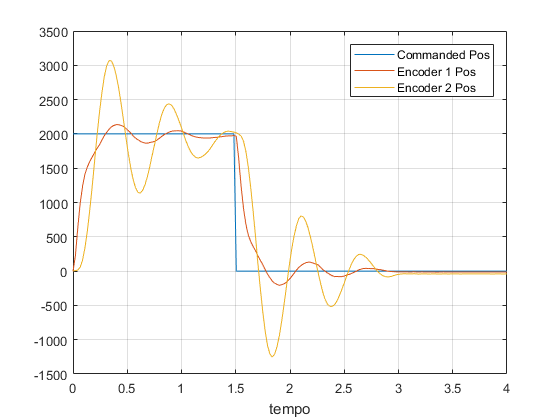
\includegraphics{q02}
\centering
\end{figure}

\pagebreak

\textbf{3.}

\begin{figure}[H]
\centering
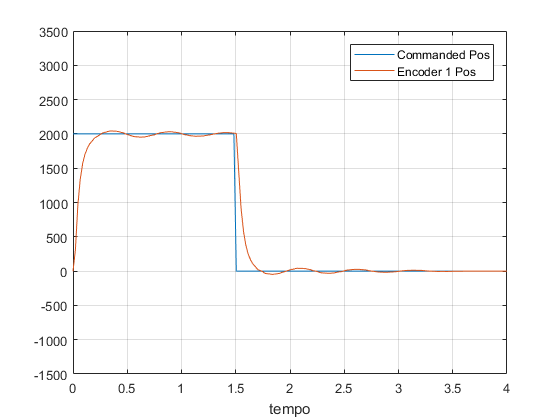
\includegraphics{q03}
\caption{$k_p = 0.4$, $k_d = 0.02$}
\end{figure}

\textbf{4.}

\begin{figure}[H]
\centering
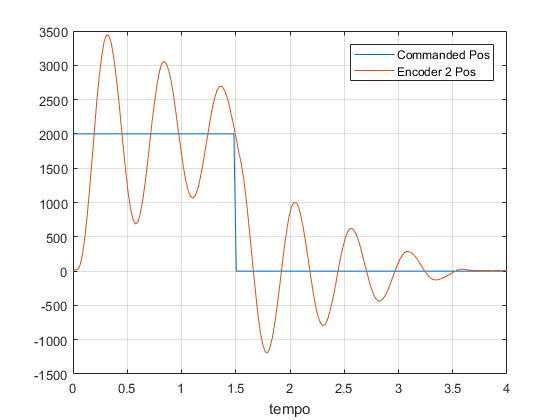
\includegraphics{q04}
\end{figure}

A característica predominante do movimento do carro \#2 é sua oscilação
que se dá de forma significativa e consideravelmente maior que no carro \#1. Na
função de transferência de $X_1\left(s\right)$ e de $X_2\left(s\right)$, há a
presença de dois pólos com parte imaginária, que fazem $X_1$ e $X_2$ oscilarem.
Esses são os pólos dominantes, que decaem mais lentamente. Porém, na função de
transferência de $X_1\left(s\right)$, existem dois zeros a mais, que estão
muito próximos a esses dois pólos, atenunando a influência dos mesmos. Com a
influência reduzida desses pólos dominantes, que estabilizam lentamente, o
sistema, então, estabiliza mais rapidamente. \\

\textbf{5.}

\begin{figure}[H]
\centering
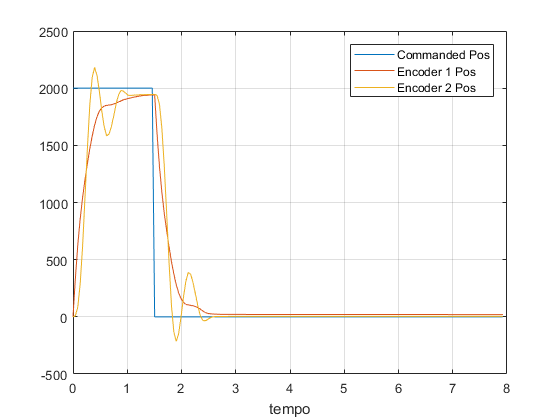
\includegraphics{q05}
\caption{$k_p = 0.105$, $k_d = 0.0225$}
\end{figure}

De maneira geral, a rigidez da mola foi menor para ambos os carros. O erro de
regime foi notavelmente maior em relação à configuração no item 3. Isso é
esperado, pois no item 3 o objetivo era tentar melhorar o controle do carro \#1,
enquanto no item 5 era de tentar melhor o controle do carro \#2. Desse modo,
espera-se que no item 5 o controle do carro \#1 seja pior, já que não é o
objetivo do item 5 controlá-lo. \\

\textbf{6.}

\begin{gather*}
  X_1\left(s\right) = \frac{N_1\left(s\right)}{D\left(s\right)} \cdot \left\{
    F_d + k_{hw} \cdot \left[k_p \cdot \left(R\left(s\right) - X_1\left(s\right)
    \right) - k_d s X_1\left(s\right)\right]\right\} \\
  X_1\left(s\right) = \frac{N_1\left(s\right)}{D\left(s\right)} \cdot \left[
    F_d - k_{hw} X_1 \left(s\right) \cdot \left(k_p + k_d s\right)\right] \\
  X_1\left(s\right) \cdot \left[1 + k_{hw}
    \frac{N_1\left(s\right)}{D\left(s\right)} \cdot \left(k_d s + k_p\right)
    \right] = \frac{N_1\left(s\right)}{D\left(s\right)} \cdot F_d \\
  \frac{X_1\left(s\right)}{F_d} = \frac{
    \frac{N_1\left(s\right)}{D\left(s\right)}}{1 + k_{hw} \left(k_d s +
    k_p\right) \frac{N_1\left(s\right)}{D\left(s\right)}}
\end{gather*}

Servo-rigidez estática:

\begin{gather*}
  = \frac{F_d}{X_1\left(s\right)} = \frac{1 + k_{hw} \left(k_d s + k_p\right)
    \frac{N_1\left(s\right)}{D\left(s\right)}}
    {\frac{N_1\left(s\right)}{D\left(s\right)}} =
    \frac{D\left(s\right)}{N_1\left(s\right)} + k_{hw}
    \left(k_d s + k_p\right) \xrightarrow{\text{s = 0}} \\
  = \frac{0}{k} + k_{hw} \left(k_d \cdot 0 + k_p\right) = k_{hw} k_p
\end{gather*}

Para o item 3, tem-se uma servo-rigidez estática de $5.89 \cdot 10^3$,
enquanto no item 5 tem-se uma servo-rigidez estática de $1.55 \cdot 10^3$.
Como esperado, a rigidez da carro \#1 é menor no item 5. \\

\textbf{7.}
Para o carro \#2:

\begin{gather*}
  \frac{X_2\left(s\right)}{X_1\left(s\right)} = \frac{N_2\left(s\right)}
    {N_1\left(s\right)} \implies X_2\left(s\right) =
    \frac{N_2\left(s\right)}{N_1\left(s\right)} \cdot \frac{
    \frac{N_1\left(s\right)}{D\left(s\right)}}{1 + k_{hw} \left(k_d s +
    k_p\right) \frac{N_1\left(s\right)}{D\left(s\right)}} =
    \frac{\frac{N_2\left(s\right)}{D\left(s\right)}}{1 + k_{hw} \left(k_d s +
    k_p\right) \frac{N_1\left(s\right)}{D\left(s\right)}}
\end{gather*}

Servo-rigidez estática:

\begin{gather*}
  = \frac{F_d}{X_1\left(s\right)} = \frac{1 + k_{hw} \left(k_d s + k_p\right)
    \frac{N_1\left(s\right)}{D\left(s\right)}}
    {\frac{N_2\left(s\right)}{D\left(s\right)}} =
    \frac{D\left(s\right)}{N_2\left(s\right)} + k_{hw}
    \left(k_d s + k_p\right) \frac{N_1\left(s\right)}{N_2\left(s\right)}
    \xrightarrow{\text{s = 0}} \\
  = \frac{0}{k} + k_{hw} \left(k_d \cdot 0 + k_p\right) \cdot \frac{k}{k} =
    k_{hw} k_p
\end{gather*}

Os valores de servo-rigidez estática no carro \#2 são os mesmos para o carro
\#1. Isso se reflete na sensação de menor rigidez também no carro \#2 para o
item 5.

\end{document}